\documentclass[Afour,times]{SIOpset}
\setcounter{secnumdepth}{3} %for section numbering

%%%%%%%%%%%%%%%%%%%%%%%%%%%%%%%%%%%%%%%%%%%%%%%%%%%%%%%%%%%%%%%%%%
%%% start document: header
%%%%%%%%%%%%%%%%%%%%%%%%%%%%%%%%%%%%%%%%%%%%%%%%%%%%%%%%%%%%%%%%%%

\begin{document}
 
% SUBSTITUTE YOUR NAME BELOW
\runninghead{Firstname Lastname, SIO 115 Spring 2020, Problem Set \#1}

\title{Problem Set \#1: The Cryosphere and its importance for climate}

% SUBSTITUTE YOUR NAME BELOW
\author{Firstname Lastname\affilnum{1}}

\thisquarter{Spring 2020}
\coursenumber{Course: SIO 115}
\coursename{\emph{Ice and the Climate System}}
\instructor{Professor: Helen A. Fricker}

% ADD YOUR MAJOR / DEPARTMENT
\affiliation{%
\affilnum{1}Your Department\\
UC San Diego\\
La Jolla, CA
}

% ADD YOUR PREFERRED EMAIL ADDRESS
\corrauth{\href{mailto:youremail@domain.xyz}{youremail@domain.xyz}}

\abstracttitle{Notes}
\begin{abstract}
Due Friday 17th January 2020.
\begin{itemize}
    \item You will be graded on your presentation and writing style as well as the content of your answer.
    \item The marks for each answer are in parentheses (Question 3 has many parts! Refer to the Week 1 lecture slides).
    \item Reference your sources, if necessary, such as the textbook \citep{marshall2011cryosphere}.
\end{itemize}
\end{abstract}
 
\maketitle

\allowdisplaybreaks
\hypersetup{colorlinks=true, linkcolor=blue}

%%%%%%%%%%%%%%%%%%%%%%%%%%%%%%%%%%%%%%%%%%%%%%%%%%%%%%%%%%%%%%%%%%
% Question 1
%%%%%%%%%%%%%%%%%%%%%%%%%%%%%%%%%%%%%%%%%%%%%%%%%%%%%%%%%%%%%%%%%%
\section{The cryosphere}

\subsection{Definition}
\question{What is the “cryosphere” and where does it exist? [2]}

% ADD YOUR ANSWER BELOW
Your answer here.

\subsection{Largest components}
\question{What is the largest component of the cryosphere in the following context:}

\subsubsection{by volume in Northern Hemisphere summer [1]:}

% ADD YOUR ANSWER BELOW
Your answer here.

\subsubsection{by volume in NH winter [1]:}

% ADD YOUR ANSWER BELOW
Your answer here.

\subsubsection{by area in NH summer [1]:}

% ADD YOUR ANSWER BELOW
Your answer here.

\subsubsection{by area in NH winter [1]:}

% ADD YOUR ANSWER BELOW
Your answer here.

\medskip
\question{Explain why (i) and (ii) are the same and (iii) and (iv) are different. [2]:}

% ADD YOUR ANSWER BELOW
Your answer here.

\subsection{Seasonal variation}
\question{Which hemisphere has the largest seasonal variation in cryosphere extent? Give some numbers to quantify your answer. [2]}

% ADD YOUR ANSWER BELOW
Your answer here. 

%%%%%%%%%%%%%%%%%%%%%%%%%%%%%%%%%%%%%%%%%%%%%%%%%%%%%%%%%%%%%%%%%%
% Question 2
%%%%%%%%%%%%%%%%%%%%%%%%%%%%%%%%%%%%%%%%%%%%%%%%%%%%%%%%%%%%%%%%%%
\section{The cryosphere in the climate system}

\subsection{Importance}
\question{What makes the cryosphere so important to climate? [2]}

% ADD YOUR ANSWER BELOW
Your answer here.

\subsection{Sensitivity}
\question{Why is the cryosphere is so sensitive to climate change? [2]}

% ADD YOUR ANSWER BELOW
Your answer here.

\subsection{Ice-albedo feedback}
\question{What is the ice-albedo feedback? [2]}

% ADD YOUR ANSWER BELOW
Your answer here.

\subsection{Interactions}
\question{Apart from the atmosphere, what is another component of the Earth system with which the cryosphere interacts, and how? [2]}

% ADD YOUR ANSWER BELOW
Your answer here.

%%%%%%%%%%%%%%%%%%%%%%%%%%%%%%%%%%%%%%%%%%%%%%%%%%%%%%%%%%%%%%%%%%
% Question 3
%%%%%%%%%%%%%%%%%%%%%%%%%%%%%%%%%%%%%%%%%%%%%%%%%%%%%%%%%%%%%%%%%%
\section{Radiative Energy Budget}
\question{The balance of energy in from the sun and energy radiated back out to space determines the global average temperature (see figure \ref{fig:radBud})}

\begin{figure}
    \centering
    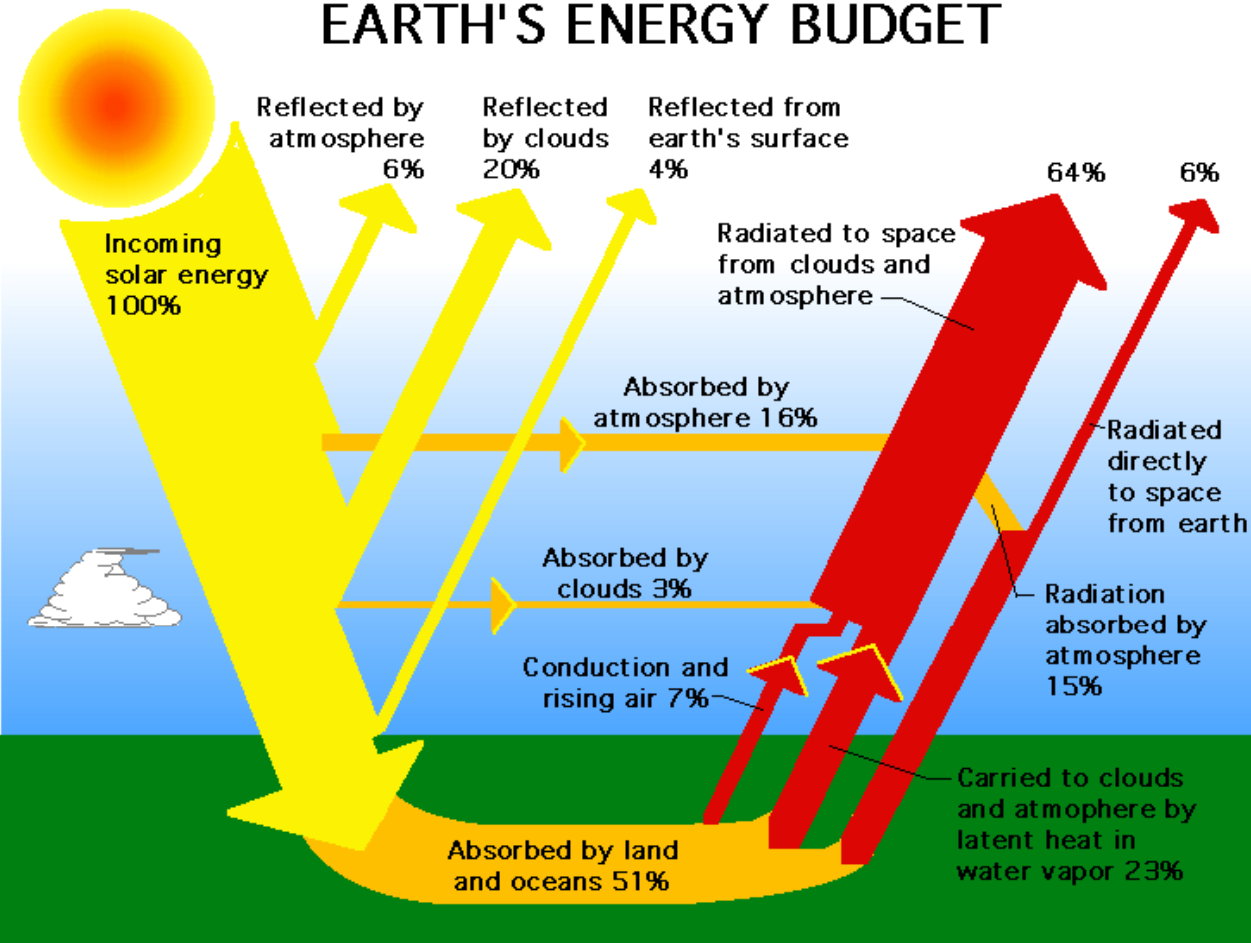
\includegraphics[width=0.48\textwidth]{figs/ps1-fig1-radiationBudget.png}
    \caption{An illustration of the Earth's radiation budget.}
    \label{fig:radBud}
\end{figure}

%%%%%%%%%%%%%%%%%%%%%%%%%%%%%%%%%%%%%%%%%%%%%%%%%%%%%%%%%%%%%%%%%%
\subsection{Incoming solar flux}
\question{The amount of energy arriving at a point in space (solar flux), $S$, varies with distance from the sun, $D$, through the Inverse Square Law:
\begin{equation} \label{eq1}
    S = S_\text{sun}\left(\frac{r_\text{sun}}{D}\right)^2
\end{equation}
where: $S_\text{sun}$ is the solar flux at the sun’s surface $(6.42 \times 10^7 \frac{W}{m^2})$ and $r_\text{sun}$ is the radius of the sun $(6.96 \times 10^5 km)$.
If Earth is $1.50 \times 10^8 km$ away from the sun, what is the solar flux arriving at the top of the Earth’s atmosphere in $\frac{W}{m^2}$? [2]}

% ADD YOUR ANSWER BELOW
Your answer here.

%%%%%%%%%%%%%%%%%%%%%%%%%%%%%%%%%%%%%%%%%%%%%%%%%%%%%%%%%%%%%%%%%%
\subsection{Total incoming solar energy}
\question{What is the total amount of energy hitting the Earth’s atmosphere in $W$? Assume the Earth’s radius is 6378 km (hint: the area of the Earth facing the sun is equal to $\pi r^2$, where $r$ is the Earth’s radius) [2]}

% ADD YOUR ANSWER BELOW
Your answer here.

%%%%%%%%%%%%%%%%%%%%%%%%%%%%%%%%%%%%%%%%%%%%%%%%%%%%%%%%%%%%%%%%%%
\subsection{Planetary albedo}
\question{Not all of this energy makes it to the Earth’s surface -- some gets reflected back to space. The amount of energy reflected divided by the total amount is the Albedo, $\alpha$. If the average albedo of the Earth’s atmosphere and surface is $\alpha = 0.3$, based on your answer for part (b), how much energy, in W, is absorbed by Earth’s atmosphere? [2]}

% ADD YOUR ANSWER BELOW
Your answer here.

%%%%%%%%%%%%%%%%%%%%%%%%%%%%%%%%%%%%%%%%%%%%%%%%%%%%%%%%%%%%%%%%%%
\subsection{Total absorbed energy}
\question{Using your calculations from parts (b) and (c), derive an equation for the total energy into the Earth’s atmosphere. The equation should have “Energy in from the sun” on the left side of the equal sign and the variables for $\pi$, earth’s radius, the solar flux and albedo on the right hand side. [2]}

% ADD YOUR ANSWER BELOW
Your answer here.

%%%%%%%%%%%%%%%%%%%%%%%%%%%%%%%%%%%%%%%%%%%%%%%%%%%%%%%%%%%%%%%%%%
\subsection{Temperature at top of the atmosphere}
\question{The flux of energy out will vary with the temperature (in Kelvin) of the earth’s atmosphere, $T_a$, as:
\begin{equation}
    \text{energy emitted to space } = \sigma T_a^4
\end{equation}
where $\sigma$ is the Stefan-Boltzmann constant $= 5.67 \times 10^{-8} \frac{W}{m^2 K^4}$. This flux will be emitted over the entire sphere of the Earth. Using your calculation for energy absorbed from the sun from part (c), calculate the temperature at the top of the Earth’s atmosphere using this equation. (Hint: the area of a sphere is $4 \pi r^2$). [2]}

% ADD YOUR ANSWER BELOW
Your answer here.

%%%%%%%%%%%%%%%%%%%%%%%%%%%%%%%%%%%%%%%%%%%%%%%%%%%%%%%%%%%%%%%%%%
\subsection{Radiative balance equation}
\question{Write an equation equating the energy absorbed by the atmosphere (energy in, from part (d)) to the energy emitted to space (energy out, part (e)) and simplify. [2]}

% ADD YOUR ANSWER BELOW
Your answer here.

%%%%%%%%%%%%%%%%%%%%%%%%%%%%%%%%%%%%%%%%%%%%%%%%%%%%%%%%%%%%%%%%%%
\subsection{Temperature at the surface}
\question{The mean temperature at the earth surface is 288 K (15\degree C). Your answer from part (e) should be quite a bit less than this. This is because energy emitted by the earth is absorbed by the atmosphere and radiated back to Earth (and outward to space), heating the surface. If we assume that the atmosphere absorbs all the energy emitted by the Earth, the balance between energy emitted by the atmosphere and the earth’s surface is:
\begin{equation} \label{eq10}
    \sigma T_s^4 = 2 \sigma T_a^4,
\end{equation}
where Ts is the temperature at the Earth’s surface (the factor of 2 is included because energy goes both upwards and downwards in the atmosphere). Using your answer for $T_a$ from part (e), calculate the temperature at the Earth’s surface. [2]}

% ADD YOUR ANSWER BELOW
Your answer here.

%%%%%%%%%%%%%%%%%%%%%%%%%%%%%%%%%%%%%%%%%%%%%%%%%%%%%%%%%%%%%%%%%%
\subsection{Atmospheric absorption}
\question{Your answer from part (g) should be greater than the true global average temperature. This is because, in reality, not all the energy emitted from the Earth is absorbed by the atmosphere. In order to get $T_s = 288$ K, you need to multiply the right hand side of your equation in part (g) by a fraction. This is the atmospheric absorption. Calculate what the absorption must be to get a global average temperature of 288 K. [2]}

% ADD YOUR ANSWER BELOW
Your answer here.

%%%%%%%%%%%%%%%%%%%%%%%%%%%%%%%%%%%%%%%%%%%%%%%%%%%%%%%%%%%%%%%%%%
\subsection{Snowball Earth}
\begin{figure}[h]
    \centering
    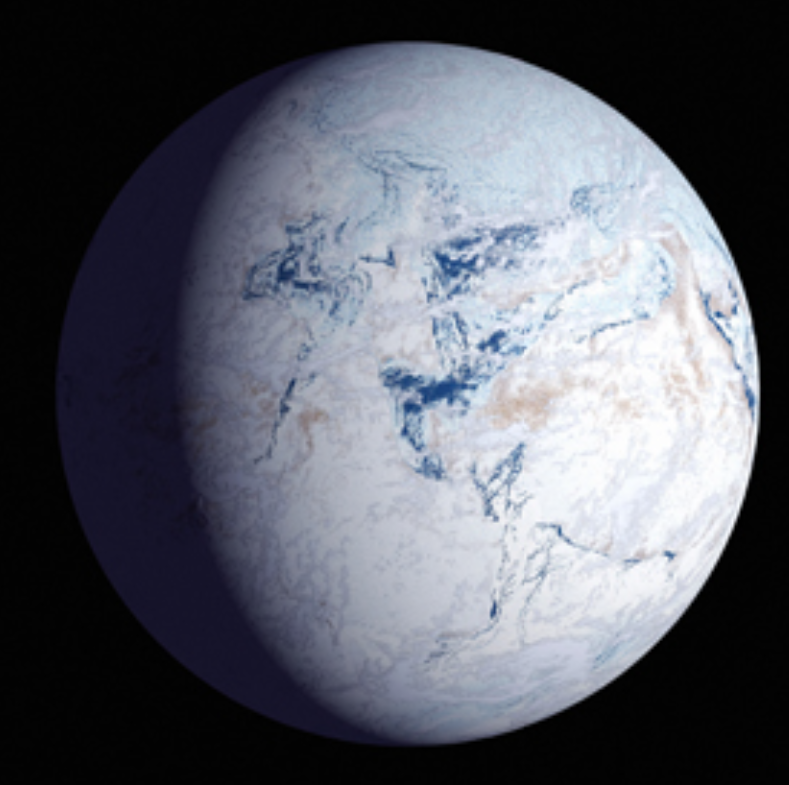
\includegraphics[width=0.25\textwidth]{figs/ps1-fig2-snowballEarth.png}
    \caption{What a "Snowball Earth" might look like.}
    \label{fig:powpowEarth}
\end{figure}

\question{ In order to have a “Snowball Earth” (the entire planet frozen), the global average surface temperature would have to be close to 0\degree C (273.15 K). Calculate (a) the atmospheric absorption and (b) the albedo needed to have a mean global temperature of 273 K. [4]}

% ADD YOUR ANSWER BELOW
Your answer here.

%%%%%%%%%%%%%%%%%%%%%%%%%%%%%%%%%%%%%%%%%%%%%%%%%%%%%%%%%%%%%%%%%%
%%% BIBLIOGRAPHY
%%%%%%%%%%%%%%%%%%%%%%%%%%%%%%%%%%%%%%%%%%%%%%%%%%%%%%%%%%%%%%%%%%
\setcitestyle{numbers}
\bibliographystyle{plainnat}
\bibliography{lit.bib} % UNCOMMENT THIS LINE IF NO REFERENCES NEEDED


%%%%%%%%%%%%%%%%%%%%%%%%%%%%%%%%%%%%%%%%%%%%%%%%%%%%%%%%%%%%%%%%%%
%%% CODE SUBMISSION (if needed...)
%%%%%%%%%%%%%%%%%%%%%%%%%%%%%%%%%%%%%%%%%%%%%%%%%%%%%%%%%%%%%%%%%%

\electronicfalse % COMMENT OUT TO SUBMIT CODE

\ifelectronic 
\section{Appendix: Code submission}

% EXAMPLE FOR GENERIC NON-HIGHLIGHTED CODE
\codeexternal{code/myCode.cpp} % enter code file name here

% EXAMPLE FOR MATLAB
\matlabexternal{code/myCode.m} % enter code file name here

% EXAMPLE FOR Python
\pythonexternal{code/myCode.py} % enter code file name here

\fi % end code submission

%%%%%%%%%%%%%%%%%%%%%%%%%%%%%%%%%%%%%%%%%%%%%%%%%%%%%%%%%%%%%%%%%%
\end{document}
%%%%%%%%%%%%%%%%%%%%%%%%%%%%%%%%%%%%%%%%%%%%%%%%%%%%%%%%%%%%%%%%%%
